\documentclass{article}
%\usepackage[spanish,activeacute]{babel}
%\usepackage[english,activeacute]{babel}
%\usepackage[latin1]{inputenc}
\usepackage[utf8]{inputenc}
\usepackage[english]{babel}

\usepackage{amsmath,amsfonts,amssymb,amstext,amsthm,amscd}
\usepackage{hyperref}
\usepackage{latexsym}
\usepackage{graphicx}
%\usepackage{subfigure}
\usepackage{subfig}
%\linespread{1.6}
\usepackage{float}
\usepackage{dcolumn}% Align table columns on decimal point(esto lo saque del ejemplo de revtex4)
\usepackage{bm}% bold math(esto lo saque del ejemplo de revtex4)
\newcounter{itemR}
\usepackage{here} %recordar usar el comando[H] para las gráficas que es el comando here en lugar de [h!]
\usepackage{fancyhdr}
%\usepackage{sidecap}
%\usepackage[spanish,activeacute]{babel}
\usepackage{multirow}
\usepackage{multicol}
\usepackage{array}
\usepackage{enumitem}
\usepackage{listings}
%\usepackage{booktabs}% para hacer tablas profesionales con \toprule

% ------------------------------------------------------------------------------------------------------------------------------------------------------

\usepackage{fancyhdr}
\setlength{\headheight}{15.2pt}
\usepackage[paperwidth=8.5in, paperheight=11.0in, top=1.0in, bottom=1.0in, left=1.0in, right=1.0in]{geometry}
\lstnewenvironment{code}{\lstset{basicstyle=\ttfamily}}{}

\pagestyle{fancyplain}
\fancyhead[LE,RO]{Actividad 3}
\fancyhead[CE,CO]{}
\fancyhead[RE,LO]{O23-LIS2012-1}
\fancyfoot[LE,RO]{\thepage}
\fancyfoot[CE,CO]{Matemáticas discretas, UDLAP}
\fancyfoot[RE,LO]{}

% ------------------------------------------------------------------------------------------------------------------------------------------------------
% ------------------------------------------------------------------------------------------------------------------------------------------------------
\begin{document}
\fancypagestyle{plain}{
   	\renewcommand{\headrulewidth}{1pt}
   	\renewcommand{\footrulewidth}{1pt}
}
\renewcommand{\footrulewidth}{1pt}
\renewcommand{\tablename}{Tabla}
\renewcommand{\figurename}{Figura}

% ------------------------------------------------------------------------------------------------------------------------------------------------------
% ------------------------------------------------------------------------------------------------------------------------------------------------------

\title{Actividad 3}
\author{\small{Erick Gonzalez Parada ID: 178145}\\
	   \small{Matemáticas discretas, Universidad de las Américas Puebla, Puebla, M\'exico}}
\date{\small{\today}}
\maketitle

% ------------------------------------------------------------------------------------------------------------------------------------------------------
% ------------------------------------------------------------------------------------------------------------------------------------------------------

\begin{abstract}
Demostración por inducción e invariante de ciclo\\
\\
\\
{\it Keywords:} inducción, ciclo
\\
\\
\end{abstract}

% ------------------------------------------------------------------------------------------------------------------------------------------------------
\section{Demostración por inducción}\label{Dpi}
\begin{equation}
  n! \geq 2^n-1
 \label{eq:1} 
\end{equation}

Se probara que la ecuación \ref{eq:1} es verdadera por inducción 

\subsection*{Paso base}\label{Pb}

\begin{figure}[H]
  \centering
  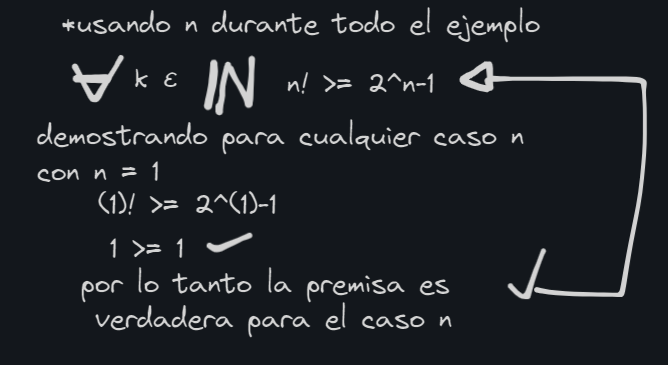
\includegraphics[scale=0.8]{../imgs/d0.png}
  \caption{paso base}
  \label{fig:1}
\end{figure}

\subsection*{Paso inductivo}\label{Pi}

\begin{figure}[H]
  \centering
  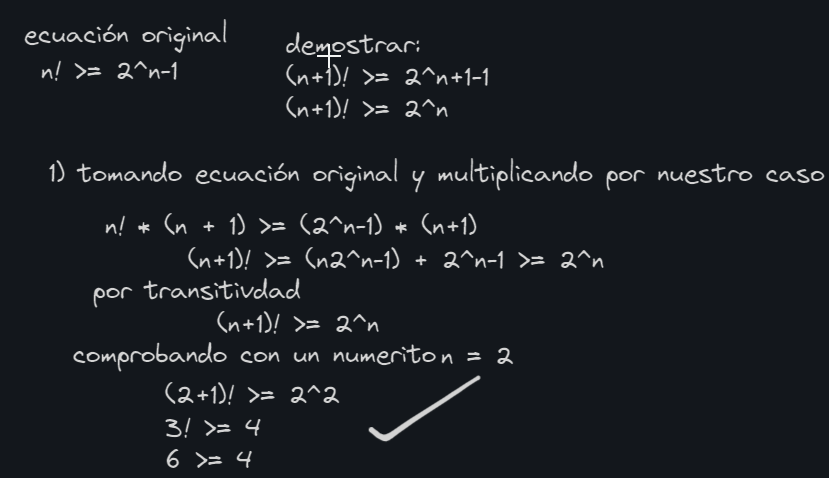
\includegraphics[scale=0.6]{../imgs/d1.png}
  \caption{paso inductivo}
  \label{fig:2}
\end{figure}

\subsection*{conclusión parte \ref{Dpi}}

La forma inductiva matemática de demostrar que una ecuación es verdadera consiste 
en básicamente hacer compatible por medio del álgebra el paso base (fig \ref{fig:1}) 
con el paso inductivo (fig \ref{fig:2}).   

\section{Invariante de ciclo merge sort}\label{Idcms}
Este algoritmo en pocas palabras divide recursivamente el problema hasta unidades individuales, luego las une de forma ordenada hacia atrás de forma recursiva.
\subsection*{código}\label{c}

\begin{code}
#include <iostream>
#include <vector>

void merge(std::vector<int>& arr, int left, int middle, int right) {
    int n1 = middle - left + 1;
    int n2 = right - middle;

    // Crear subarreglos temporales
    std::vector<int> L(n1);
    std::vector<int> R(n2);

    // Copiar datos a los subarreglos L[] y R[]
    for (int i = 0; i < n1; i++) {
        L[i] = arr[left + i];
    }
    for (int j = 0; j < n2; j++) {
        R[j] = arr[middle + 1 + j];
    }

    // Fusionar los subarreglos en arr[left..right]
    int i = 0, j = 0, k = left;
    while (i < n1 && j < n2) {
        if (L[i] <= R[j]) {
            arr[k] = L[i];
            i++;
        } else {
            arr[k] = R[j];
            j++;
        }
        k++;
    }

    // Copiar los elementos restantes de L[], si los hay
    while (i < n1) {
        arr[k] = L[i];
        i++;
        k++;
    }

    // Copiar los elementos restantes de R[], si los hay
    while (j < n2) {
        arr[k] = R[j];
        j++;
        k++;
    }
}

void mergeSort(std::vector<int>& arr, int left, int right) {
    if (left < right) {
        int middle = left + (right - left) / 2;

        // Ordenar la primera mitad y la segunda mitad
        mergeSort(arr, left, middle);
        mergeSort(arr, middle + 1, right);

        // Combinar las mitades ordenadas
        merge(arr, left, middle, right);
    }
}

int main() {
    std::vector<int> arr = {12, 11, 13, 5, 6, 7};
    int arrSize = arr.size();

    std::cout << "Arreglo original: ";
    for (int i = 0; i < arrSize; i++) {
        std::cout << arr[i] << " ";
    }
    std::cout << std::endl;

    mergeSort(arr, 0, arrSize - 1);

    std::cout << "Arreglo ordenado: ";
    for (int i = 0; i < arrSize; i++) {
        std::cout << arr[i] << " ";
    }
    std::cout << std::endl;

    return 0;
}
\end{code}
\subsection*{Invariante de ciclo}\label{Idc}
esta la encontramos (en el caso del código) en antepenúltimo while loop, básicamente
el más importante del algoritmo, en donde juntamos el array izquierdo ya ordenado con el 
array derecho, por ende la invariante de ciclo es esa: mientras estamos juntando en un 
array "final" o "resultante" array[left] \& array[right] están ordenando, teniendo así, 
la solución parcial ya que nuestro objetivo es ordenar todo.  
\section{Invariante de ciclo en algoritmo erróneo}\label{Idceae}

\subsection*{algoritmo incorrecto}\label{algoI}
En el siguiente algoritmo (código en python) se forzó un error y se va analizar que le 
sucede que a la invariante de ciclo.

\begin{code}
  def accSum(list):
    for element in list:
        sum = 0
        sum = sum + element
    return sum

nums = [1,2,3]
print(accSum(nums))
\end{code}

Para los principiantes programando quizá no sea tan obvio el error al principio
pero es muy sencillo, nuestra invariante de ciclo es que lo que ya hemos explorado en el
array ya tenemos la suma parcial de eso, por ende tenemos la solución parcial aquí significan 
básicamente la misma cosa.\\
Sin embargo debido a un error de semántica en la implementación del algoritmo alteramos gravemente
nuestra invariante ya que estamos reseteando nuestra variable donde guardamos esta promesa de
la invariante que es que siempre tendremos la suma (y solución) parcial presente.


\subsection*{algoritmo correcto}\label{algo}
\begin{code}
  def accSum(list):
  sum = 0
    for element in list:
        sum = sum + element
    return sum

nums = [1,2,3]
print(accSum(nums))
\end{code}


\end{document}